\documentclass{beamer}
\usepackage{minted}
\usepackage[skins,minted,breakable]{tcolorbox}
\usepackage[english]{babel}
\usepackage{subcaption}
\usetikzlibrary{matrix,backgrounds}
\usepackage{multirow}
\usepackage{hyperref}
\usepackage{multicol}
\usepackage{adjustbox}
\usepackage{soul}
\usepackage{graphicx}% http://ctan.org/pkg/graphicx
\usepackage{booktabs}% http://ctan.org/pkg/booktabs

\graphicspath{ {./img/} }
\selectlanguage{english}
\usepackage[utf8]{inputenc}
\usetheme{PaloAlto}
\setbeamerfont{section in sidebar}{size=\fontsize{2}{4}\selectfont}
\setbeamerfont{subsection in sidebar}{size=\fontsize{2}{3}\selectfont}
\setbeamerfont{subsubsection in sidebar}{size=\fontsize{2}{2}\selectfont}

\setbeamerfont{section in toc}{size=\footnotesize}
\setbeamerfont{subsection in toc}{size=\scriptsize}
\setbeamerfont{subsubsection in toc}{size=\tiny}

\hypersetup{
    urlcolor=cyan           % color of external links
}




\title{Media Informatic Systems}
\date{$7^{th}$ December 2018}
\subtitle{Image recognition task}

\author{Carlos Sánchez Páez}

\makeatletter
  \setbeamertemplate{sidebar \beamer@sidebarside}%{sidebar theme}
  {
    \beamer@tempdim=\beamer@sidebarwidth%
    \advance\beamer@tempdim by -6pt%
    \insertverticalnavigation{\beamer@sidebarwidth}%
    \vfill
    \ifx\beamer@sidebarside\beamer@lefttext%
    \else%
      \usebeamercolor{normal text}%
      \llap{\usebeamertemplate***{navigation symbols}\hskip0.1cm}%
      \vskip2pt%
    \fi%
}%
\makeatother

\subject{Media Informatic Systems}
\AtBeginSection[]
  {
     \begin{frame}<beamer>
     \frametitle{Index}
     \tableofcontents[currentsection]
     \end{frame}
  }
\AtBeginSubsection[]
{
  \begin{frame}<beamer>{Index}
    \tableofcontents[currentsection,currentsubsection]
  \end{frame}
}
\AtBeginSubsubsection[]
{
  \begin{frame}<beamer>{Index}
    \tableofcontents[currentsection,currentsubsection]
  \end{frame}
}

% Let's get started
\begin{document}
\centering
\begin{frame}
 \titlepage
\end{frame}

\begin{frame}{Index}
 \tableofcontents
 % You might wish to add the option [pausesections]
\end{frame}

\section{Description of the task}

\begin{frame}[fragile]{Description of the task}
 \vspace{1.8cm}
 \begin{enumerate}
  \item Convolutional neural network.
  \item Keras framework with TensorFlow backend.
  \item Python 3.6.
  \item NVIDIA 960M GPU (1 505 GFLOPS).
 \end{enumerate}
 \vspace{1.6cm}
 \begin{figure}[H]
  
\includegraphics[scale=0.17]{img/keras.jpg}
  \hspace{0.8cm}
  
\includegraphics[scale=0.03]{img/python.png}  \hspace{1cm}
  
\includegraphics[scale=0.1]{img/cuda.jpg}
 \end{figure}

\end{frame}

\section{Dataset}
\begin{frame}[fragile]{CIFAR100}
 \begin{enumerate}
  \item<+-> 60 000 32x32 color images (RGB).
  \item<+-> 100 classes.
  \item<+-> 600 images per class.
        \begin{enumerate}
         \item<+-> 500 training.
         \item<+-> 100 testing.
        \end{enumerate}
  \item<+-> Best accuracy: 75.72\%
 \end{enumerate}

\end{frame}

\begin{frame}[fragile]{Classes in the dataset}
 \begin{table}
  \centering
  \scalebox{0.65}{
   \begin{tabular}{|c|c|}
    \hline
    \textbf{Superclass}            & \textbf{Classes}                                      \\
    \hline
    aquatic mammals                & beaver, dolphin, otter, seal, whale                   \\
    \hline
    fish                           & aquarium fish, flatfish, ray, shark, trout            \\
    \hline

    flowers                        & orchids, poppies, roses, sunflowers, tulips           \\
    \hline
    food containers                & bottles, bowls, cans, cups, plates                    \\
    \hline
    fruit and vegetables           & apples, mushrooms, oranges, pears, sweet peppers      \\
    \hline
    household electrical devices   & clock, computer keyboard, lamp, telephone, television \\
    \hline
    household furniture            & bed, chair, couch, table, wardrobe                    \\
    \hline
    insects                        & bee, beetle, butterfly, caterpillar, cockroach        \\
    \hline
    large carnivores               & bear, leopard, lion, tiger, wolf                      \\
    \hline
    large man-made outdoor things  & bridge, castle, house, road, skyscraper               \\
    \hline
    large natural outdoor scenes   & cloud, forest, mountain, plain, sea                   \\
    \hline
    large omnivores and herbivores & camel, cattle, chimpanzee, elephant, kangaroo         \\
    \hline
    medium-sized mammals           & fox, porcupine, possum, raccoon, skunk                \\
    \hline
    non-insect invertebrates       & crab, lobster, snail, spider, worm                    \\
    \hline
    people                         & baby, boy, girl, man, woman                           \\
    \hline
    reptiles                       & crocodile, dinosaur, lizard, snake, turtle            \\
    \hline
    small mammals                  & hamster, mouse, rabbit, shrew, squirrel               \\
    \hline
    trees                          & maple, oak, palm, pine, willow                        \\
    \hline
    vehicles 1                     & bicycle, bus, motorcycle, pickup truck, train         \\
    \hline
    vehicles 2                     & lawn-mower, rocket, streetcar, tank, tractor          \\
    \hline
   \end{tabular}
  }
 \end{table}

\end{frame}


\section{Preprocessing}

\begin{frame}[fragile]{Preprocessing I}
 \begin{figure}[H]
  \centering
  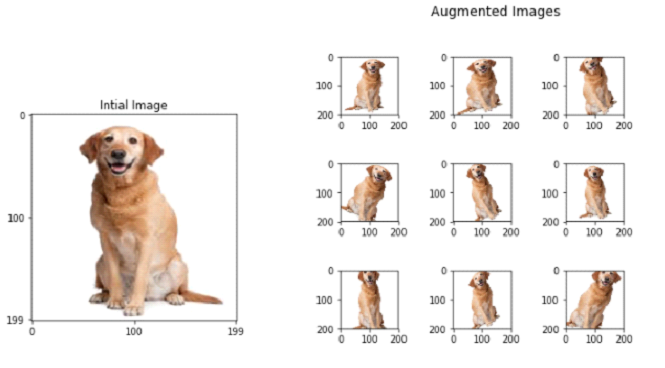
\includegraphics[scale=0.45]{img/image_augmentation.png}
 \end{figure}
\end{frame}

\begin{frame}[fragile]{Preprocessing II}
 \begin{figure}[H]
  \centering
  \begin{minted}[fontsize=\small]{python}
   datagen = ImageDataGenerator(
       featurewise_center=False,
       samplewise_center=False,
       featurewise_std_normalization=False,
       samplewise_std_normalization=False,
       zca_whitening=False,
       rotation_range=0,
       width_shift_range=0.1,
       height_shift_range=0.1,
       horizontal_flip=True,
       vertical_flip=True)
   \end{minted}
 \end{figure}
\end{frame}

\section{Structure of the net}

\begin{frame}[fragile]{Structure of the net I}
 \begin{multicols}{2}

  \begin{enumerate}
   \item<+-> Convolutional layer (128 filters)
   \item<+-> Convolutional layer (128 filters)
   \item<+-> Max Pooling layer (2x2)
   \item<+-> Dropout layer
   \item<+-> Convolutional layer (256 filters)
   \item<+-> Convolutional layer (256 filters)
   \item<+-> Max Pooling layer (2x2)
   \item<+-> Dropout layer
   \item<+-> Convolutional layer (512 filters)
   \item<+-> Convolutional layer (512 filters)
   \item<+-> Max Pooling layer (2x2)
   \item<+-> Dropout layer
   \item<+-> Flatten layer
   \item<+-> Fully connected layer (1024 neurons)
   \item<+-> Dropout layer
   \item<+-> Output layer (10 neurons)
  \end{enumerate}
 \end{multicols}


\end{frame}

\begin{frame}[fragile]{Structure of the net II}
 \begin{minted}[fontsize=\scriptsize,breaklines=true]{python}
  model = Sequential()

  model.add(Conv2D(128, (3, 3), padding='same',
                   input_shape=x_train.shape[1:], activation='elu'))
  model.add(Conv2D(128, (3, 3), activation='elu'))
  model.add(MaxPooling2D(pool_size=(2, 2)))
  model.add(Dropout(0.25))

  model.add(Conv2D(256, (3, 3), padding='same', activation='elu'))
  model.add(Conv2D(256, (3, 3), activation='elu'))
  model.add(MaxPooling2D(pool_size=(2, 2)))
  model.add(Dropout(0.25))

  model.add(Conv2D(512, (3, 3), padding='same', activation='elu'))
  model.add(Conv2D(512, (3, 3), activation='elu'))
  model.add(MaxPooling2D(pool_size=(2, 2)))
  model.add(Dropout(0.25))

  model.add(Flatten())
  model.add(Dense(1024, activation='elu'))
  model.add(Dropout(0.5))
  model.add(Dense(parameters.NUM_CLASSES, activation='softmax'))

  \end{minted}
\end{frame}

\section{Neural network development}

\begin{frame}[fragile]{Neural network development}
 \begin{enumerate}
  \item<+-> Calibration of parameters.
        \begin{enumerate}
         \item<+-> Learning rate.
         \item<+-> Number of epochs.
         \item<+-> Batch size.
        \end{enumerate}
  \item<+-> Find the maximum global accuracy.
 \end{enumerate}
\end{frame}

\begin{frame}[fragile]{200 epochs training}
 \begin{figure}[H]
  \centering
  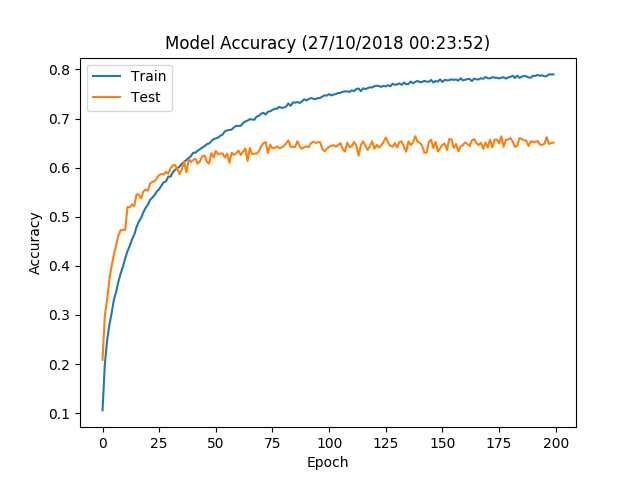
\includegraphics[scale=0.55]{img/accuracy.png}
 \end{figure}
\end{frame}
\begin{frame}[fragile]{200 epochs training}
 \begin{figure}[H]
  \centering
  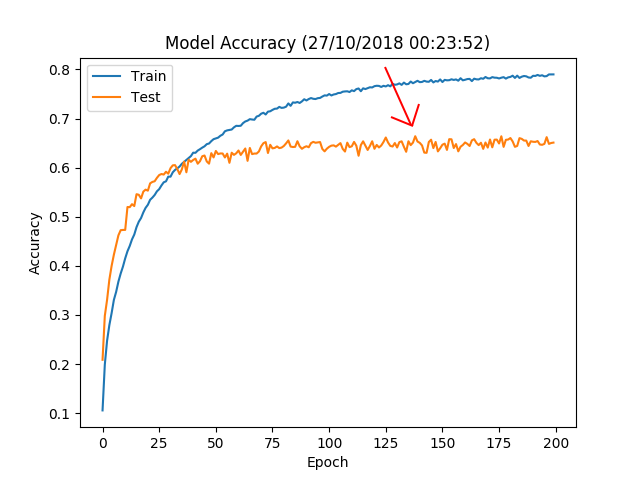
\includegraphics[scale=0.4]{img/accuracy_arrow.png}
 \end{figure}
\end{frame}



\begin{frame}[fragile]{139 epochs training}
 \begin{figure}[H]
  \centering
  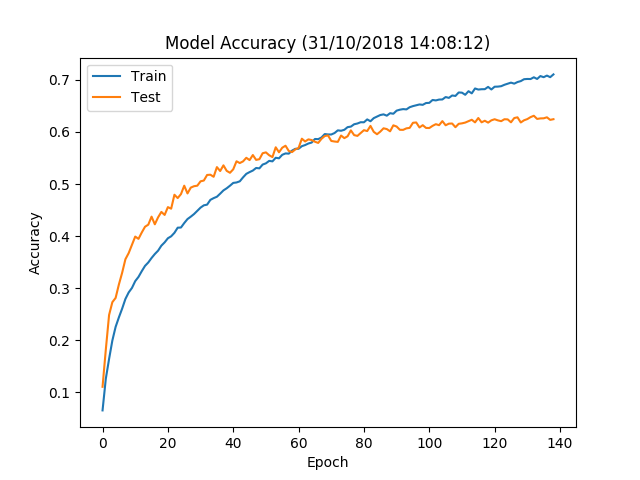
\includegraphics[scale=0.55]{img/accuracy_139.png}
 \end{figure}
\end{frame}

\begin{frame}[fragile]{200 epochs training}
 \begin{figure}[H]
  \centering
  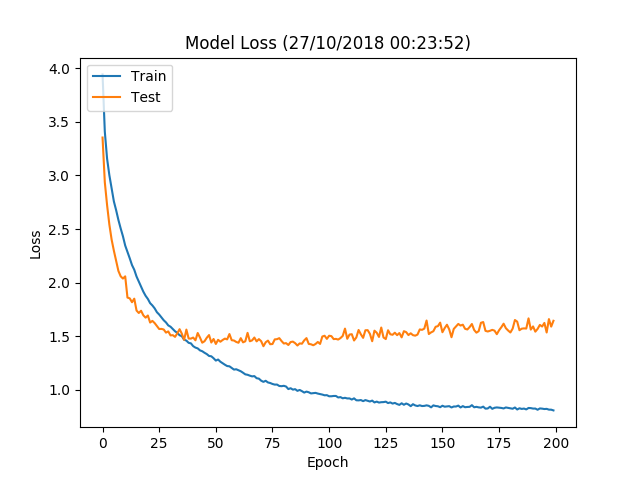
\includegraphics[scale=0.55]{img/loss.png}
 \end{figure}
\end{frame}


\begin{frame}[fragile]{139 epochs training}
 \begin{figure}[H]
  \centering
  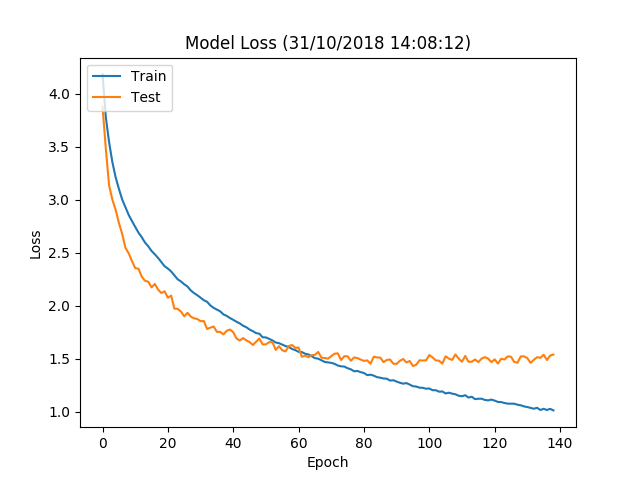
\includegraphics[scale=0.55]{img/loss_139.png}
 \end{figure}
\end{frame}



\section{Final results}

\begin{frame}[fragile]{139 epochs training}
 \begin{enumerate}
  \item Validation accuracy: 0.6187 \%
  \item Validation loss: 1.5597 \%
 \end{enumerate}
\end{frame}

\section{Examples}

\begin{frame}[fragile]{Crocodile prediction}
 \scalebox{0.8}{
  \begin{minipage}{\textwidth}
   \begin{figure}[H]
    \centering
    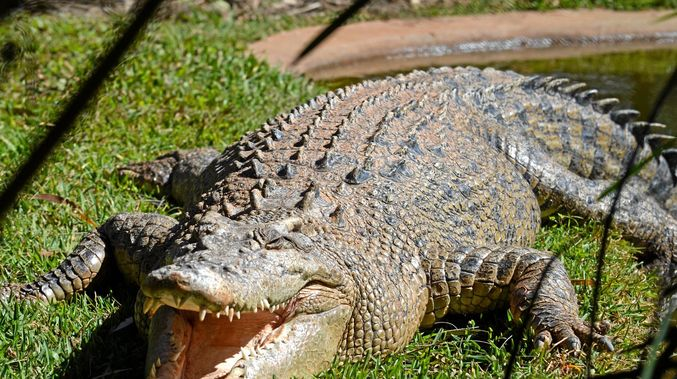
\includegraphics[scale=0.25]{crocodile.jpg}
    \hspace{2em}
    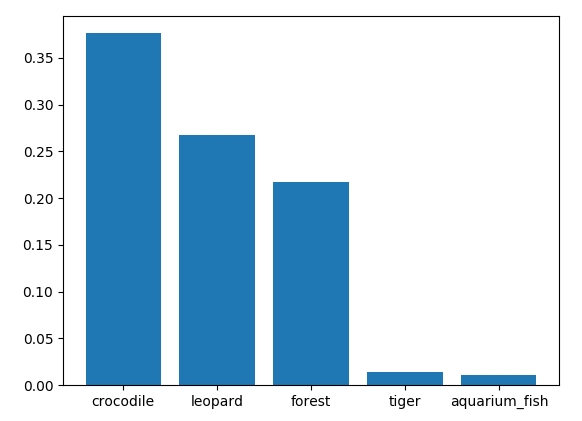
\includegraphics[scale=0.4]{crocodile_prediction.jpg}
   \end{figure}
  \end{minipage}
 }
\end{frame}

\begin{frame}[fragile]{Bee prediction}
 \scalebox{0.8}{
  \begin{minipage}{\textwidth}
   \begin{figure}[H]
    \centering
    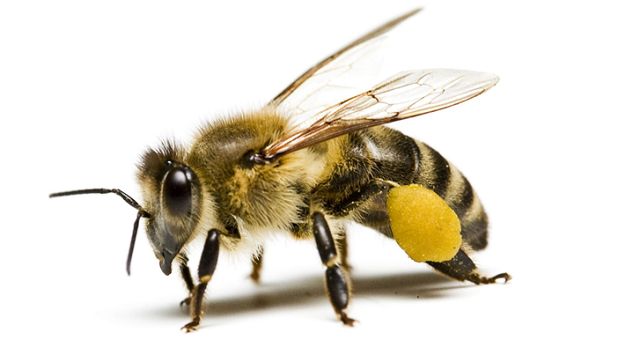
\includegraphics[scale=0.3]{bee.png}
    \hspace{2em}
    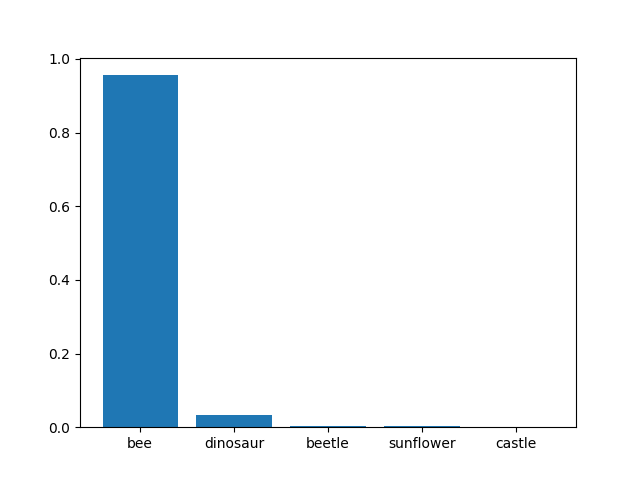
\includegraphics[scale=0.5]{bee_prediction.png}
   \end{figure}
  \end{minipage}
 }
\end{frame}

\begin{frame}[fragile]{Porcupine prediction}
 \scalebox{0.8}{
  \begin{minipage}{\textwidth}
   \begin{figure}[H]
    \centering
    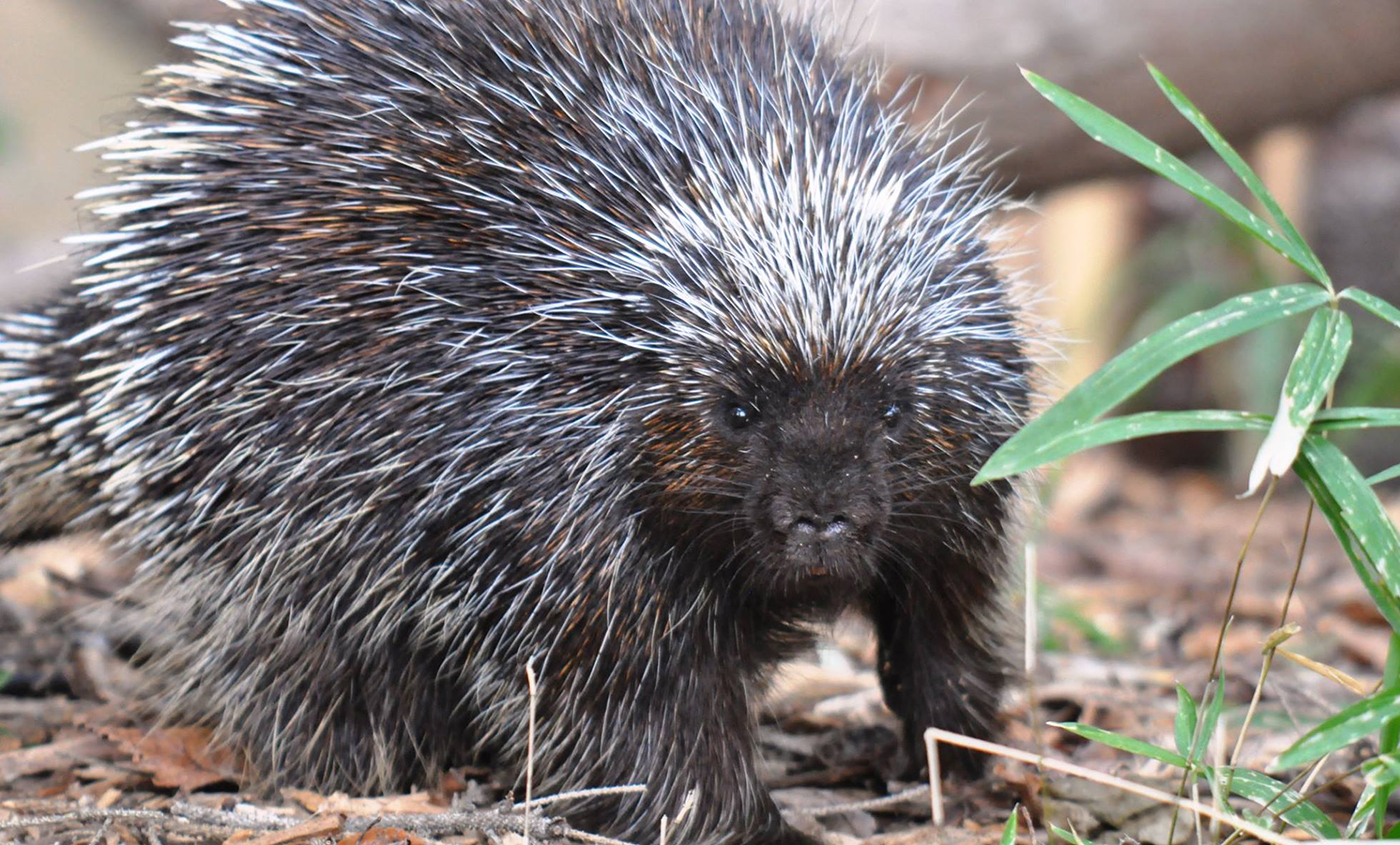
\includegraphics[scale=0.45]{porcupine.jpg}
    \hspace{2em}
    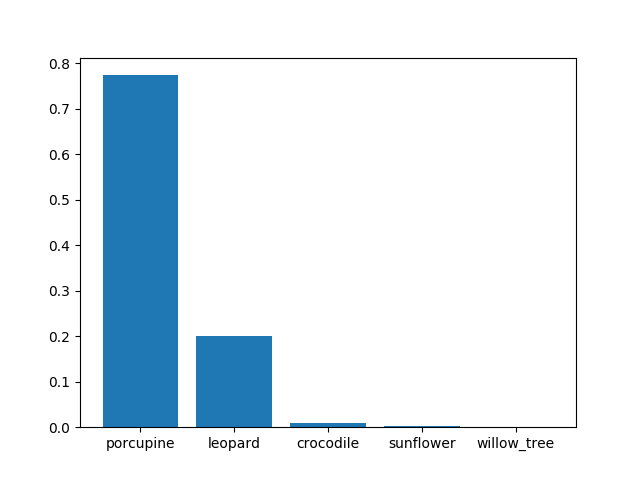
\includegraphics[scale=0.5]{porcupine_prediction.png}
   \end{figure}
  \end{minipage}
 }
\end{frame}

\begin{frame}[fragile]{Bear prediction}
 \scalebox{0.8}{
  \begin{minipage}{\textwidth}
   \begin{figure}[H]
    \centering
    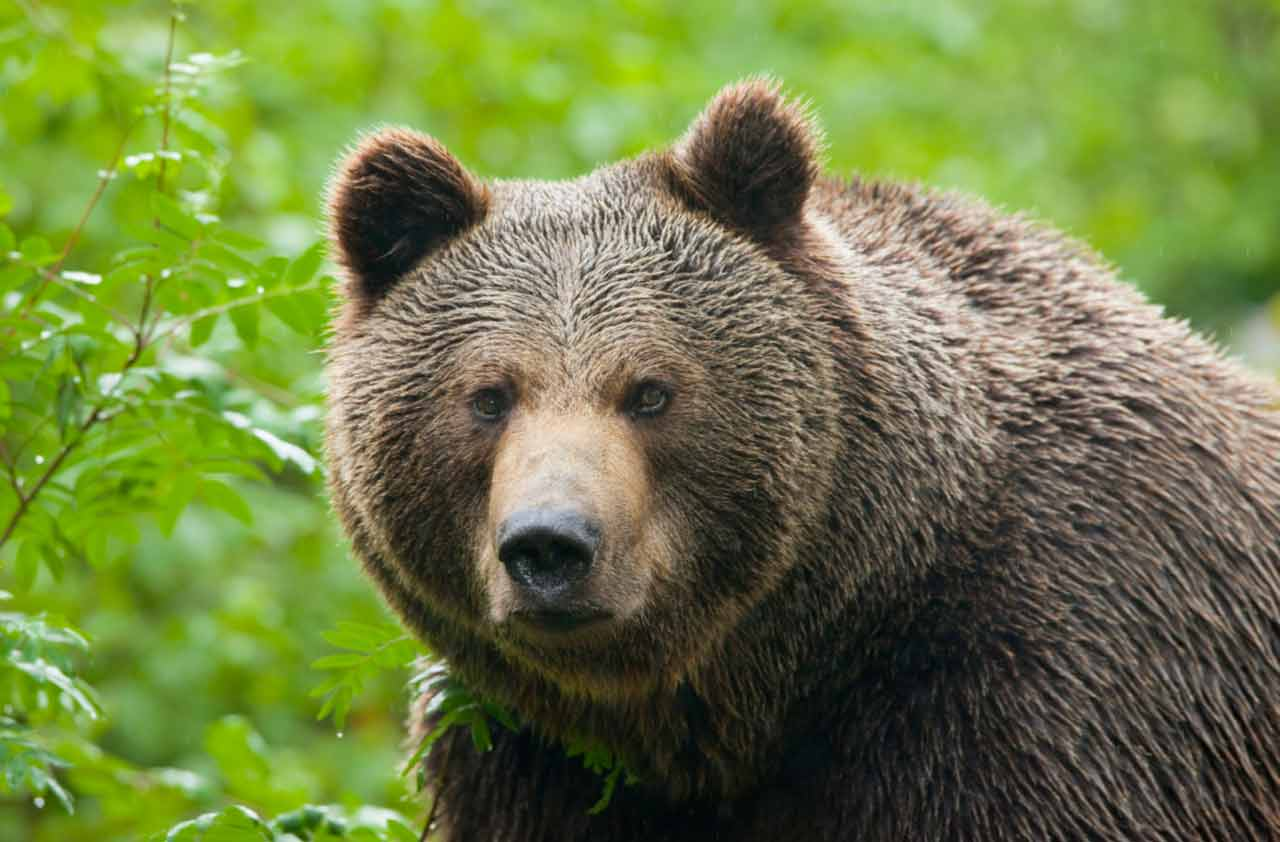
\includegraphics[scale=0.15]{bear.jpg}
    \hspace{2em}
    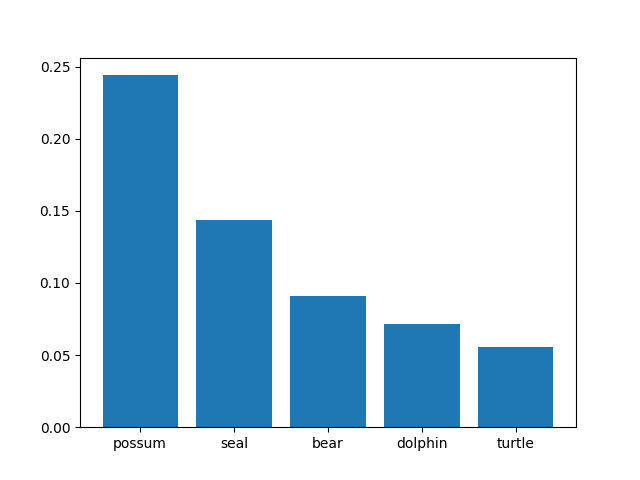
\includegraphics[scale=0.45]{bear_prediction.png}
   \end{figure}
  \end{minipage}
 }
\end{frame}

\section{Bibliography}

\begin{frame}[allowframebreaks]{Bibliography}
\footnotesize

  \begin{thebibliography}{8}
  \setbeamertemplate{bibliography item}[online]

   \bibitem{Keras documentation}
   Keras documentation
   \\\texttt{https://keras.io/}

   \bibitem{Moodle}
   Moodle
   \\\texttt{https://elearning.tmit.bme.hu/login/index.php}

   \bibitem{Tensorflow Tutorial}
   Tensorflow Tutorial
   \\\texttt{https://cv-tricks.com/tensorflow-tutorial/\\training-convolutional-neural-network-for\\-image-classification/}

   \bibitem{Some Datasets}
   Some Datasets
   \\\texttt{https://www.analyticsvidhya.com/blog/2018/03/\\comprehensive-collection-deep-learning-datasets/}


   \bibitem{Understanding Convolutions}
   Understanding Convolutions
   \\\texttt{https://towardsdatascience.com/intuitively-understanding\\-convolutions-for-deep-learning-1f6f42faee1}

   \bibitem{Deep neural net tutorial}
   Deep neural net tutorial
   \\\texttt{https://medium.com/@tifa2up/image-classification\\-using-\\deep-neural-networks-a-beginner-friendly-\\approach-using-tensorflow-94b0a090ccd4}

   \bibitem{Caltech-101 dataset}
   Caltech-101 dataset
   \\\texttt{http://www.vision.caltech.edu/Image\_Datasets/Caltech101/}


   \bibitem{Caltech-256 dataset}
   Caltech-256 dataset
   \\\texttt{http://www.vision.caltech.edu/Image\_Datasets/Caltech256/}


   \bibitem{TensorFlow tutorial}
   TensorFlow tutorial
   \\\texttt{https://cv-tricks.com/artificial-intelligence/deep-\\learning/deep-learning-frameworks/\\tensorflow/tensorflow-tutorial/}

   \bibitem{Basic classification tutorial with Tensorflow}
   Basic classification tutorial with Tensorflow
   \\\texttt{https://www.tensorflow.org/tutorials/keras/basic\_\\classification}


   \bibitem{Keras tutorial}
   Keras tutorial
   \\\texttt{https://medium.com/@vijayabhaskar96/tutorial-image\\-classification-with-keras-flow-from-\\directory-and-generators-95f75ebe5720}

   \bibitem{Another Keras tutorial}
   Another Keras tutorial
   \\\texttt{https://machinelearningmastery.com/tutorial-\\first-neural-network-python-keras/}

   \bibitem{Doubts resolution}
   Doubts resolution
   \\\texttt{https://stackoverflow.com/}

  \end{thebibliography}

\end{frame}

\begin{frame}[fragile]
 \begin{center}
  \Huge
  Thanks for your attention!
 \end{center}
 \vspace{2cm}
 Source code available at \textcolor{blue}{\url{http://www.github.com/csp98}}
 \vspace{1cm}
 \begin{figure}[H]
  \centering
  
\includegraphics[scale=0.05]{github-mark.png}
 \end{figure}

\end{frame}

\end{document}
